%%% srs.tex --- 

%% Author: Baishampayan Ghose <b.ghose@gnu.org.in>
%% Version: $Id: srs.tex,v 0.0 2006/04/06 19:19:42 ghoseb Exp$


\documentclass[12pt,a4paper]{article}
\usepackage[debugshow,final]{graphicx}
\newcommand{\VS}{\textit{Vyasa}}

% %% SET ALL MARGINS 1 INCH ---------------------------------------
% \oddsidemargin  0.0in
% \evensidemargin 0.0in
% \textwidth      6.27in
% \headheight     14.5pt
% \topmargin      0.0in
% \textheight     8.90in
% %% --------------------------------------------------------------

\usepackage{newcent}
\title {Vyasa -- A simple, multilingual, cross-platform text editor \\ \small{\texttt{http://vyasa.berlios.de/}}}
\author {\large{Baishampayan Ghose\footnote{\texttt{b.ghose@gnu.org}},
    Aatif Haider\footnote{\texttt{aatif.haider@gmail.com}}, \textit{et
      al.}} \\\small{T.E.~ Computer Science \&{} Engineering}\\ \small{\textsc{D.Y. Patil College of Engineering \&{} Technology,}}
\\ \small{\textsc{Kolhapur, Maharashtra}}}

\begin{document}
\maketitle
\tableofcontents
\listoffigures
%%%%##########################################################################
\newpage
\section{Introduction}
The {\bfseries Software Requirements Specifications} (SRS) of
\VS{} --- a simple, multilingual and cross-platform text editor
are laid out in this document. It is expected to be useful for
installation, configuration, documentation purposes by end-users and developers.

\subsection{Purpose}
This SRS documents the requirement specifications of the version 1.0 of
\VS. The requirements for installing and using \VS{} are explained in
detail here. Also the various parts of the code are explained here for
the future developer.

\subsection{Scope of the Project}
\VS{} is intended to be a very simple and easy to use text-editor. It
has excellent multilingual display capabilities which will enable the
end-user to use it for typing text in various languages. It supports
state-of-the-art Indic Language support via the Pango rendering
library. \VS{} is written in the Python programming language which is
also an excellent Object Oriented programming language and is incredibly
easy to use and extend. \VS{} uses the GTk+ GUI toolkit for the User
Interface which is also a Free \&{} Open Source cross-platform GUI
toolkit.
\VS{} can be a very good tool for people who want to use a light-weight
and feature rich text-editor for creating multilingual documents. It can
also be useful for students who want to learn Python programming.

\subsection{Definitions, Acronyms, Abbreviations \&{} References}
\begin{enumerate}
\item Python -- Python is an object-oriented, interpreted programming
  language with dynamic semantics [http://www.python.org/]
\item GTk+ -- GTk+ is a cross platform GUI toolkit [http://www.gtk.org/]
\item \VS{} -- \VS{} is a simple, multilingual text editor
  [http://vyasa.berlios.de/]
\item Pango -- Pango is a text rendering library for GTk+
\end{enumerate}

\subsection{Overview of the Document}
This document provides the users, developers of \VS{} a bird's eye view
of the software in general and information about installing, configuring
and enhancing \VS{} in particular.

The mechanics of installing \VS{} are provided in detail as well as the
requirements for using it.


\section{Overall Description}
\subsection{Product Perspective}
\VS{} is a simple and lightweight text-editor written in Python \&{}
GTk+. One of the main aims of \VS{} is to provide the user with an easy
and effective way to input multilingual text. In future it will also
support automatic syntax highlighting and indenting for programming
languages. \VS{} is also cross-platform as in it can be run on any
platfrom that supports Python \&{} GTk+ libraries.

\subsection{Product Functions}
\begin{enumerate}
\item Create and open plain text documents
\item Create plain text documents with Unicode text in different
  languages
\item Use as an editor for programming
\item Use as a viewer / pager for text files
\end{enumerate}

\subsection{User Characteristics}
\begin{enumerate}
\item \VS{} Users --- End-users can use \VS{} by directly executing the
  file ``run'' as \texttt{./run} from the console or by double-clicking on
  the ``run'' file.
\item \VS{} Developers --- The code for \VS{} is located in the
  \texttt{vyasa.py} file. Most of the code is very straight-forward and
  self-descriptive. The use-interface definitions are located in the
  \texttt{vyasa.glade} file. The latest source code can be downloaded
  from the \VS{} \textit{Subversion} repository located at
  \texttt{http://svn.berlios.de/wsvn/vyasa}.
\item \VS{} Documenters --- The code and this SRS will be pretty useful
  for documenters for documenting \VS.
\end{enumerate}

\subsection{General Constraints}
The implementation constraints of \VS{} are limited to the performance
of the Python interpreter itself. But since Python is itself written in
very hightly optimised C, the performance issues won't be obvious in any
of the modern day computers.

The API of the GTk+ library may change in the newer versions. In that
case we can easily update \VS{} to suit the changes made in the GTk+
library itself.

\subsection{Assumptions \&{} Dependencies}
It's assumed that the system where \VS{} will be run will already have
Python and the GTk+ toolkit pre-installed.
\VS{} has been tested to work fine on the following two harwares
configurations ---
\begin{enumerate}
\item Intel Pentium 4 Mobile 1.8 GHz.\\768 MiB of RAM\\Ubuntu Linux 6.06 ``Dapper Drake'' Development version.
\item AMD Athlon 64FX 2.4 GHz.\\2 GiB RAM\\Debian GNU/Linux 3.1 ``Sarge''.
\end{enumerate}
\VS{} has no memory limitations and it can work just fine on systems
with 64 MiB RAM.

\section{Specific Requirements}
\VS{} will need the Python interpreter and the GTk+ GUI toolkit for its
execution. Apart from that it has no other requirements.

\subsection{External Interface Requirements}
Not applicable.

\subsubsection{User Interfaces}
The GTk+ GUI toolkit is needed for the user interface.
\begin{figure}[ht]
\centering
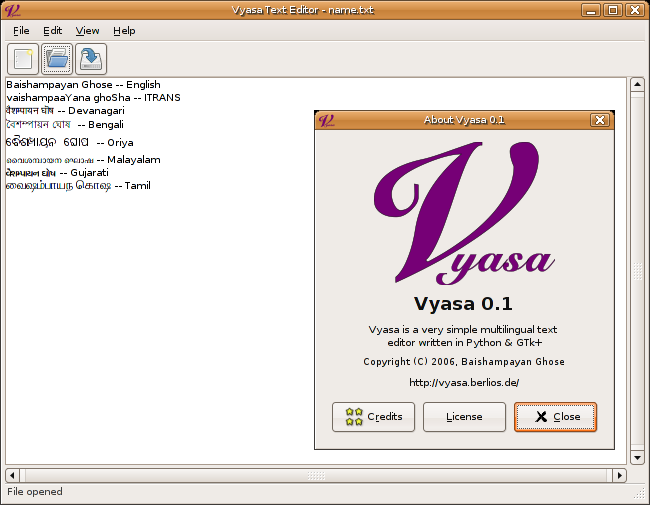
\includegraphics[width=5.5in]{vyasa-screenshot.png}
\caption{\VS{} in action}
\end{figure}

\subsubsection{Hardware Interfaces}
Not Applicable.

\subsubsection{Software Interfaces}
The Python interpreter and standard libraries with the GTk+ toolkit
serve the purpose of providing the interface.
\VS{} needs Python v 2.4.3 or later and GTk+ library 2.8.x or later.

\subsubsection{Communication Interfaces}
Not applicable.

\subsection{Functional Requirements}
\VS{} as such has no specific functional requirements.

\subsection{Performance Requirements}
Not applicable.

\subsection{Design Constraints}
\VS{} being a very simple application has no design constraints as
such. Its design flaws if any, are directly inherited from either the
GTk+ toolkit or Python itself. The chances of any of the above happening
are very less as both of them are enterprise grade applications.

\subsection{Attributes}

\subsubsection{Software Quality}
\VS{} is developed using the \textit{Bazaar}-style development
model. The development of the project is totally open to the public and
thus everybody will be able to inspect the code and find bugs if any. So
in a way we can say that a certain level of Software Quality is assured
in \VS{}.

\subsubsection{Business Rules}
\VS{} is released under the \textit{GNU General Public
  License} v2. Everybody is thus free to copy, share, modify \&{}
redistribute the software provided that the derivative works are also
released under GNU GPLv2. Business rules are not applicable otherwise.

\subsubsection{Data Migration}
The data created in \VS{} can be very easily migrated to work with
different editors and platforms.

\subsection{Other Requirements}
Not applicable.



%%%%##########################################################################

\end{document}

%%% Local Variables: 
%%% mode: latex
%%% TeX-master: t
%%% End: 
